\documentclass[border=10mm]{standalone}
\usepackage{tikz}
\usetikzlibrary{arrows, shapes.gates.logic.US, shapes.gates.logic.IEC, calc}

\tikzset{
    my-and-gate/.style={
        and gate US, draw, rotate=0, logic gate inputs=nn
    },
    my-xor-gate/.style={
      xor gate US, draw, rotate=0, logic gate inputs=nn
    },
    my-branch/.style={
      fill, shape=circle, minimum size=3pt, inner sep=0pt
    },
}

\begin{document}

\resizebox{15cm}{!}{

    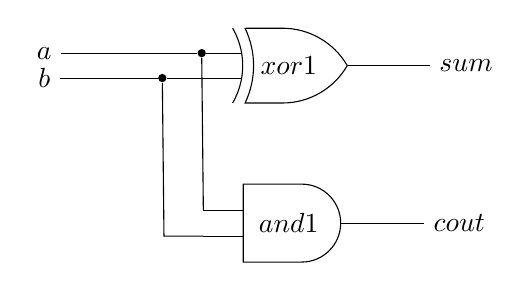
\begin{tikzpicture}[label distance=2mm]

        % XOR, WIRES AND CONNECTOR POINTS
        \node[my-xor-gate]     (XOR1)    at (0,0)                        {\normalsize $xor1$};
        \coordinate[my-branch] (XOR1IN1) at ($(XOR1.input 1) + (-.5, 0)$) {};
        \coordinate[]          (XOR1IN2) at ($(XOR1.input 2) + (-.5, 0)$) {};
        \coordinate[]          (XOR1OUT) at ($(XOR1.output)  + (.5, 0)$)  {};
        \draw (XOR1.input 1) -- (XOR1IN1);
        \draw (XOR1.input 2) -- (XOR1IN2);
        \draw (XOR1.output)  -- (XOR1OUT);

        % INPUTS
        \node[] (A)    at ($(XOR1IN1) + (-2, 0)$)  {\normalsize $a$};
        \node[] (B)    at ($(XOR1IN2) + (-2, 0)$)  {\normalsize $b$};

        %B WIRE CONNECTOR POINTS
        \coordinate[my-branch]  (BCONNECT) at ($(XOR1IN2) + (-.5, 0)$) {};

        % INPUT CONNECTIONS
        \draw (A) -- (XOR1IN1);
        \draw (B) -- (BCONNECT);
        \draw (BCONNECT) -- (XOR1IN2);

        % AND, WIRES AND CONNECTOR POINTS
        \node[my-and-gate]     (AND1)    at ($(XOR1) + (0, -2)$) {\normalsize $and1$};
        \coordinate[]          (AND1IN1) at ($(AND1.input 1) + (-.5, 0)$) {};
        \coordinate[]          (AND1IN2) at ($(AND1.input 2) + (-.5, 0)$) {};
        \coordinate[]          (AND1OUT) at ($(AND1.output)  + (.5, 0)$)  {};
        \draw (AND1.input 1) -- (AND1IN1);
        \draw (AND1.input 2) -- (AND1IN2);
        \draw (AND1.output)  -- (AND1OUT);

        % INTERNAL WIRES
        \draw (XOR1IN1) -- (AND1IN1);
        \draw (BCONNECT) -- ($(AND1IN2) + (-.5, 0)$) -- (AND1IN2);

        % OUTPUTS
        \node[] (SUM)    at ($(XOR1OUT) + (1, 0)$)  {\normalsize $sum$};
        \node[] (COUT)   at ($(AND1OUT) + (1, 0)$)  {\normalsize $cout$};

        % OUTPUT CONNECTIONS
        \draw (XOR1OUT) -- (SUM);
        \draw (AND1OUT) -- (COUT);

    \end{tikzpicture}
}

\end{document} 
